\documentclass[12pt, a4paper]{article}

\usepackage{array}
\usepackage[portuguese]{babel}
\usepackage{chngpage}
\usepackage{float}
\usepackage[a4paper, margin=2cm]{geometry}
\usepackage{graphicx}
\usepackage{hyperref}
\usepackage{setspace}
\usepackage{xcolor}

\title{\Huge \textbf{Computação Gráfica \\ \Large Trabalho Prático -- Fase I}}
\date{2 de março 2025}
\author{Grupo \textbf{\color{red} TODO}}

\begin{document}

\begin{center}
    
\includegraphics[width=0.25\textwidth]{res/cover/EE-C.eps}
\end{center}

\chardef\_=`_
\onehalfspacing
\setlength{\parskip}{\baselineskip}
\setlength{\parindent}{0pt}
\def\arraystretch{1.5}

{\let\newpage\relax\maketitle}
\maketitle
\thispagestyle{empty}

\vspace*{\fill}

\begin{adjustwidth}{-2cm}{-2cm} % These values only need to be large enough to center the table
    \begin{center}
        \begin{tabular}{>{\centering}p{0.25\textwidth}
                        >{\centering}p{0.25\textwidth}
                        >{\centering}p{0.25\textwidth}
                        >{\centering\arraybackslash}p{0.25\textwidth}}
            
\includegraphics[width=3.5cm]{res/cover/A104437.png} &
            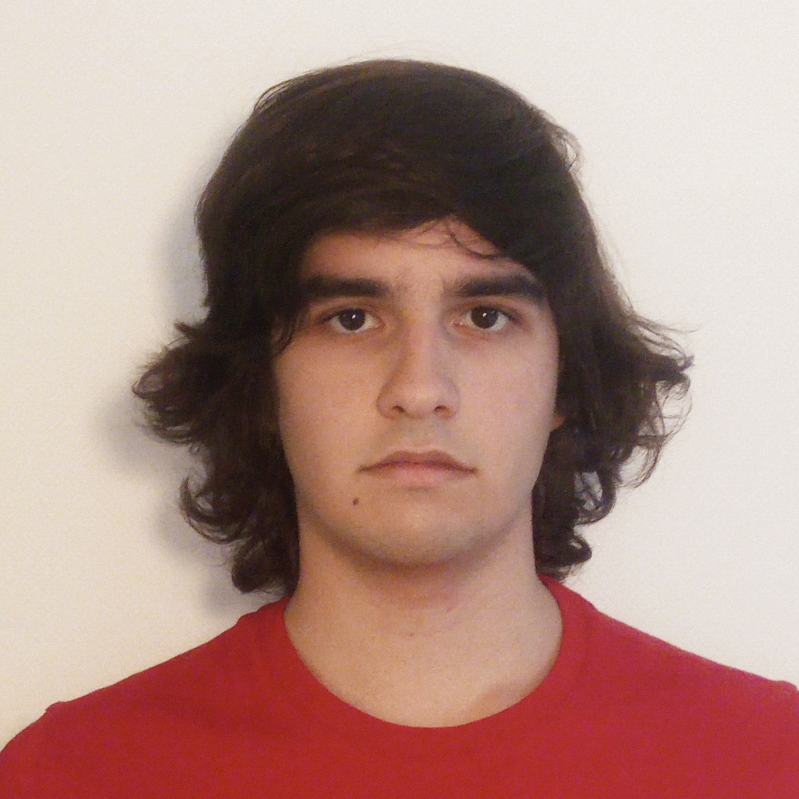
\includegraphics[width=3.5cm]{res/cover/A104348.png} &
            
\includegraphics[width=3.5cm]{res/cover/A90817.png} &
            
\includegraphics[width=3.5cm]{res/cover/A104179.png} \\

            Ana Oliveira & Humberto Gomes & Mariana Cristino & Sara Lopes \\
            A104437      & A104348        & A90817           & A104179
        \end{tabular}
    \end{center}
\end{adjustwidth}

\pagebreak

\begin{abstract}
    \textbf{\color{red} TODO - resumo}
\end{abstract}

\section{\emph{Generator}}

\textbf{\color{red} TODO - \emph{generator}}

\section{\emph{Engine}}

\textbf{\color{red} TODO - \emph{engine}}

\subsection{Torus}

Matematicamente, as coordenadas de um ponto do \emph{torus} são definidas do seguinte modo
\cite{torus}:

$$
x = (-R + r \cos \phi) \cos \theta
\hspace{1cm}
y = r \sin \phi
\hspace{1cm}
z = (-R + r \cos \phi) \sin \theta
$$

$R$ e $r$ são os parâmetros dados para a geração do \emph{torus}, os raios maior e menor,
respetivamente. Os ângulos $\theta$ e $\phi$ variam ambos no intervalo $[0, 2\pi]$.

O ângulo $\theta$ define a rotação do ponto em torno do eixo central do torus, percorrendo o
círculo principal de raio $R$. Assim, ao variar $\theta$, o ponto desloca-se ao longo do anel do
torus, mantendo-se sempre na mesma posição relativa dentro do tubo. Já o ângulo $\phi$ determina a
posição do ponto dentro da secção transversal do tubo, que tem raio $r$. Ao variar $\phi$, o ponto
descreve um movimento circular dentro do tubo, movendo-se ao longo da circunferência menor do torus.

Para gerar uma nuvem de pontos uniformemente distribuídos, dividem-se os ângulos em fatias
($slices$) e segmentos ($stacks$), utilizando:

$$
\theta_i = i \cdot \frac{2\pi}{slices}, \quad i \in \{0, 1, \ldots, slices-1\}
$$

$$
\phi_j = j \cdot \frac{2\pi}{stacks}, \quad j \in \{0, 1, \ldots, stacks-1\}
$$

Assim, o torus é gerado iterando sobre os valores inteiros possíveis de $i$ e $j$, incrementando
primeiro $j$ e só depois $i$, o que dá origem à nuvem de pontos desejada.

Depois de gerados, os vértices são agrupados nos triângulos que compõem a superfície do torus. Para
isso, considera-se um vértice de referência, como $P_1$, juntamente com o vértice adjacente na
mesma fatia ($P_2$) e os dois vértices correspondentes na fila seguinte da grelha ($P_3$ e $P_4$).
Este processo repete-se para todos os vértices aplicáveis, garantindo que cada célula quadrangular
seja subdividida em dois triângulos. A figura seguinte ilustra esse processo, mostrando a estrutura
da malha e a organização dos triângulos resultantes.

\begin{figure}[H]
    \centering
    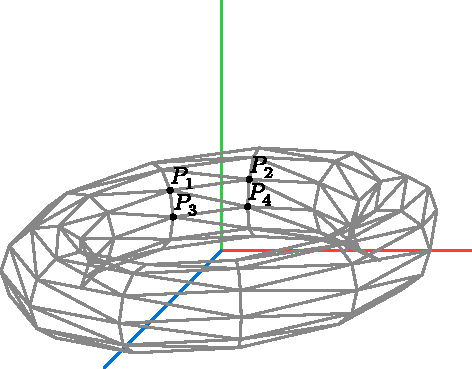
\includegraphics[width=0.4\textwidth]{res/figures/TorusTriangle.pdf}
    \caption{Triângulos de um torus gerado. As faces ocultas não são apresentadas.}
\end{figure}

Deseja-se que os triângulos do \emph{torus} estejam voltados para fora, pelo que os seus vértices
devem estar ordenados na ordem contrária à dos ponteiros do relógio. Para os quatro pontos
apresentados acima, os triângulos gerados são os seguintes:

$$
T_1 = (P_1, P_2, P_4)
\hspace{1cm}
T_2 = (P_1, P_4, P_3).
$$

O \emph{torus} é a única superfície côncava gerada, o que trás problemas relativos à orientação das
suas normais. As normais de todas as faces apontam para "fora"{} do \emph{torus}, ou seja, as das
faces interiores ("do buraco"{}) apontam para o centro do \emph{torus}, e as das faces exteriores
apontam no sentido contrário.

Idealmente, a parte interna do \emph{torus} não deveria ser visível quando este é observado de fora,
pois a própria geometria bloquearia essa visão. No entanto, como apenas os contornos das faces são
desenhados, e a direção das normais é o único critério utilizado de momento para determinar se uma
face é ou não desenhada, pode ocorrer um efeito onde a parte interna do \emph{torus} é visível, como
mostra a figura abaixo. Esse fenómeno acontece porque as normais da parte interna apontam para a
câmara, tal como as normais das faces que a deveriam cobrir.

\textbf{\color{red} TODO - figura com a cena do torus}

Este problema será mitigado na fase 4 do trabalho, onde a superfície dos polígonos será preenchida
por completo, e as faces internas do \emph{torus} serão cobertas pelas faces externas.

\section{Resultados obtidos}

\textbf{\color{red} TODO - resultados}

\section{Conclusão e Trabalho Futuro}

\textbf{\color{red} TODO - conclusão}

\begingroup
\section{Bibliografia}
\renewcommand{\section}[2]{}

\begin{thebibliography}{9}
    \bibitem{torus}
        "Torus."{} Wolfram MathWorld. Accessed: Mar. 1, 2025. [Online.] Available:
        \url{https://mathworld.wolfram.com/Torus.html}
\end{thebibliography}
\endgroup

\end{document}
